Consider the \emph{fourth order} partial differential equation
\[ u_t(x,t) = u_{xx}(x,t) - u_{xxxx}(x,t)\]
with so-called \emph{hinged} boundary conditions
\[ u(0,t) = u_{xx}(0,t) = u(1,t) = u_{xx}(1,t) = 0\]
and initial condition (that should satisfy the boundary conditions)
\[ u(x,0) = u_0(x).\]
(This equation is related to a model that arises in the study of thin films.)

      To solve this PDE, we introduce the linear
      operator $L: C^4_H[0,1] \to C[0,1]$, where 
      \[ Lu = -u'' + u''''\]
      and 
     \[ C^4_H[0,1] = \{ u \in C^4[0,1], u(0)=u''(0)=u(1)=u''(1)=0\}\]
      is the set of $C^4$ functions that satisfy the hinged boundary conditions.

\begin{enumerate}
\item The operator $L$ has eigenfunctions 
       \[ \psi_n(x) = \sqrt{2} \sin(n \pi x), \qquad n=1, 2, \ldots.\]
      Use this fact to compute a formula for the eigenvalues $\lambda_n$,
       $n=1,2, \ldots.$
    
\item Suppose the initial condition $u_0(x)$ is expanded in the form
      \[ u_0(x) = \sum_{n=1}^\infty a_n(0) \psi_n(x).\]
      Briefly describe how one can write the solution to the 
      PDE $u_t = u_{xx}-u_{xxxx}$ as an infinite sum.

\item Suppose the initial data is given by
\[ u_0(x) = (x-x^2) \sin(3\pi x)^2,\]
with associated coefficients
\[ a_n(0) = \left\{ \begin{array}{cl} 
      \displaystyle{{432\sqrt{2} (n^4-18n^2 + 216) \over (36n-n^3)^3 \pi^3}}, & \mbox{$n$ odd}; \\[.75em]
      0, & \mbox{$n$ even}.
\end{array}\right. \]
Write a program (you may modify your earlier codes) to compute the
solution you describe in part~(b) up to seven terms in the infinite sum.
At each time $t=0$; $10^{-5}$; $2\times 10^{-5}$; $4 \times 10^{-5}$, produce a plot comparing
the sum of the first 1, 5, and 7 terms of the series.
For example, at time $t=0$, your plot should appear as shown below.
(Alternatively, you can produce attractive 3-dimensional plots over the time interval
$t\in [0, 4\times10^{-5}]$ using 1, 5, and 7 terms in the series.)

\ifthenelse{\boolean{showsols}}{}{\vfill \hfill \emph{continued on next page\ldots}}

\begin{center}
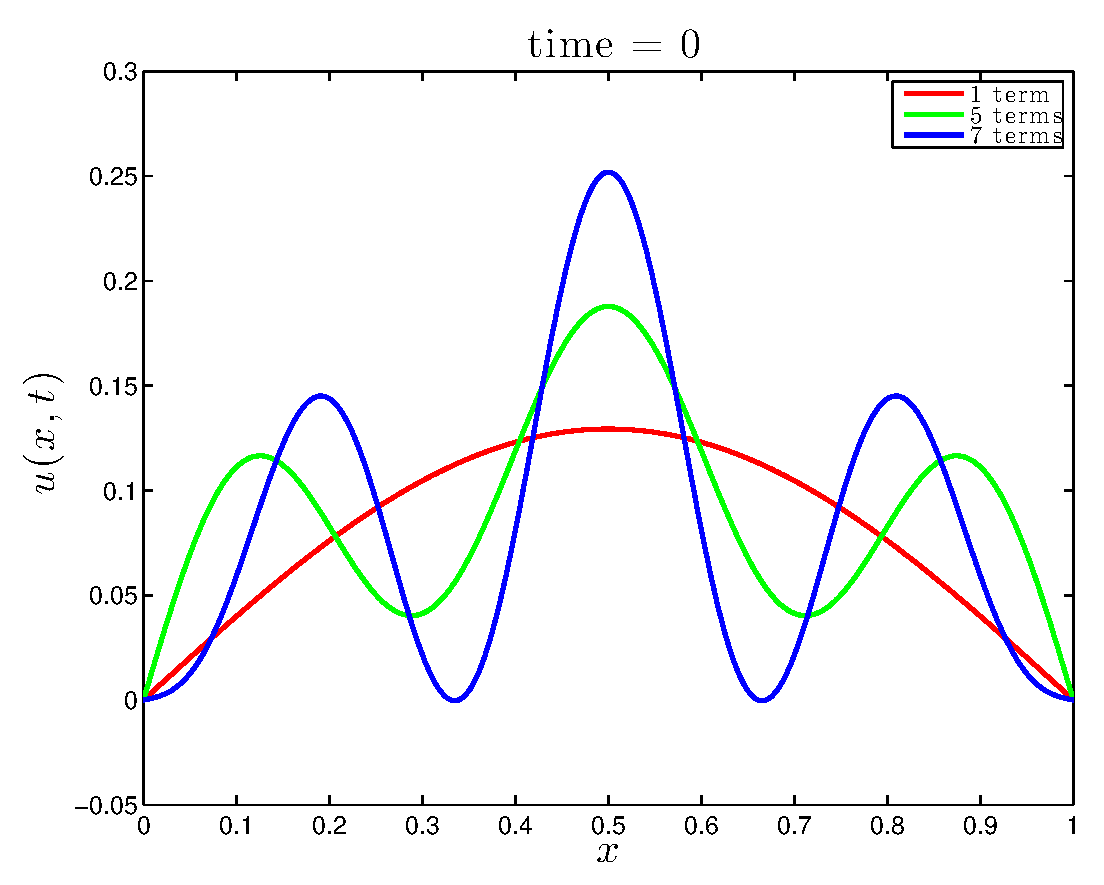
\includegraphics[scale=0.5]{fourth_a}
\end{center}
\end{enumerate}

%%%%%%%%%%%%%%%%%%%%%%%%%%%%%%%%%%%%%%%%%%%%%%%%%%%%%%%%%%%%%%%%%%%%%%%%%%%%%%%%
\ifthenelse{\boolean{showsols}}{\begin{solution}
\begin{enumerate}
\item Given the eigenfunctions $\psi_n$, we simply apply $L$ to $\psi_n$ to 
      compute $\lambda_n \psi_n$:
     \begin{eqnarray*}
          L \psi_n(x) &=& -\psi_n''(x) + \psi_n''''(x)  \\[0.25em]
                      &=& -{d^2 \over dx^2} (\sqrt{2} \sin(n\pi x)) + {d^4\over dx^4}(\sqrt{2} \sin(n\pi x)) \\[.25em]
                      &=& n^2\pi^2 \sqrt{2} \sin(n\pi x) + n^4\pi^4 \sqrt{2}\sin(n\pi x)\\[.25em]
                      &=& (n^2\pi^2 + n^4\pi^4) (\sqrt{2} \sin(n\pi x) \\[.25em]
                      &=& \lambda_n \psi_n(x).
     \end{eqnarray*} 
     Thus, we identify $\lambda_n = n^2\pi^2 + n^4\pi^4$ for $n=1,2,\ldots$.

\item Following the prodedure outlined in class, we look for a solution of the form
         \[ u(x,t) = \sum_{n=1}^\infty a_n(t) \psi_n(x).\]
      Substituting this equation into the differential equation, we obtain
         \begin{eqnarray*}
           \sum_{n=1}^\infty a_n'(t) \psi_n(x) 
               &=& \sum_{n=1}^\infty a_n(t) (\psi_n''(x) - \psi_n''''(x)) \\[0.25em]
               &=& \sum_{n=1}^\infty -\lambda_n a_n(t) \psi_n(x).
         \end{eqnarray*}
      Taking an inner product of both sides with $\psi_k$ and using the orthonormality 
      of the eigenfunctions, we obtain the scalar differential equations
      \[ a_k'(t) = -\lambda_k a_k(t),\]
      which has the solution
      \[ a_k(t) = e^{-\lambda_k} a_k(0).\]
      Thus, the solution can be written in the series
      \begin{eqnarray*}
              u(x,t) &=& \sum_{n=1}^\infty e^{-\lambda_n t} a_n(0) \psi_n(x) \\[0.5em]
                     &=& \sum_{n=1}^\infty \sqrt{2} e^{-(n^2\pi^2 + n^4\pi^4)t} a_n(0) \sin(n\pi x).
      \end{eqnarray*}
      [GRADERS: students need only write down one of these series solutions for $u(x,t)$; 
       they need not include the derivation.]

\item  Plots for the four requested times are shown below.
\begin{center}
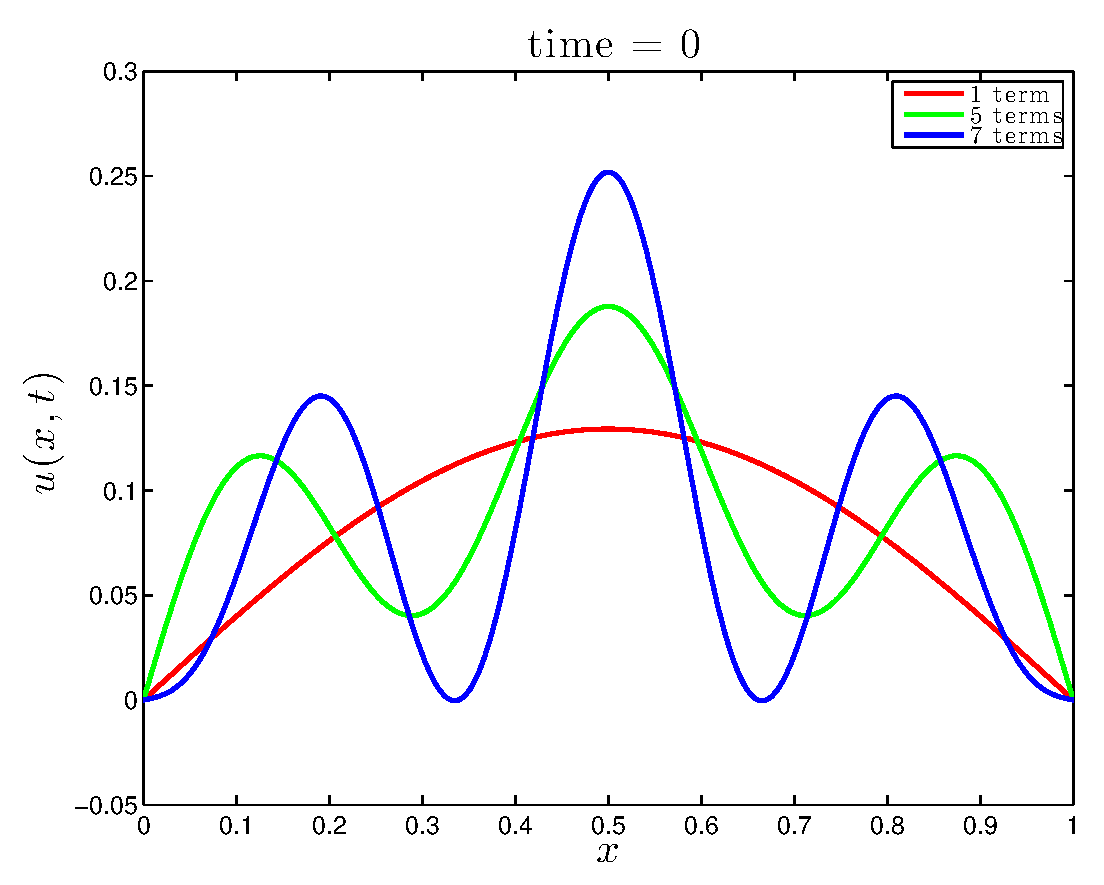
\includegraphics[scale=0.4]{fourth_a}
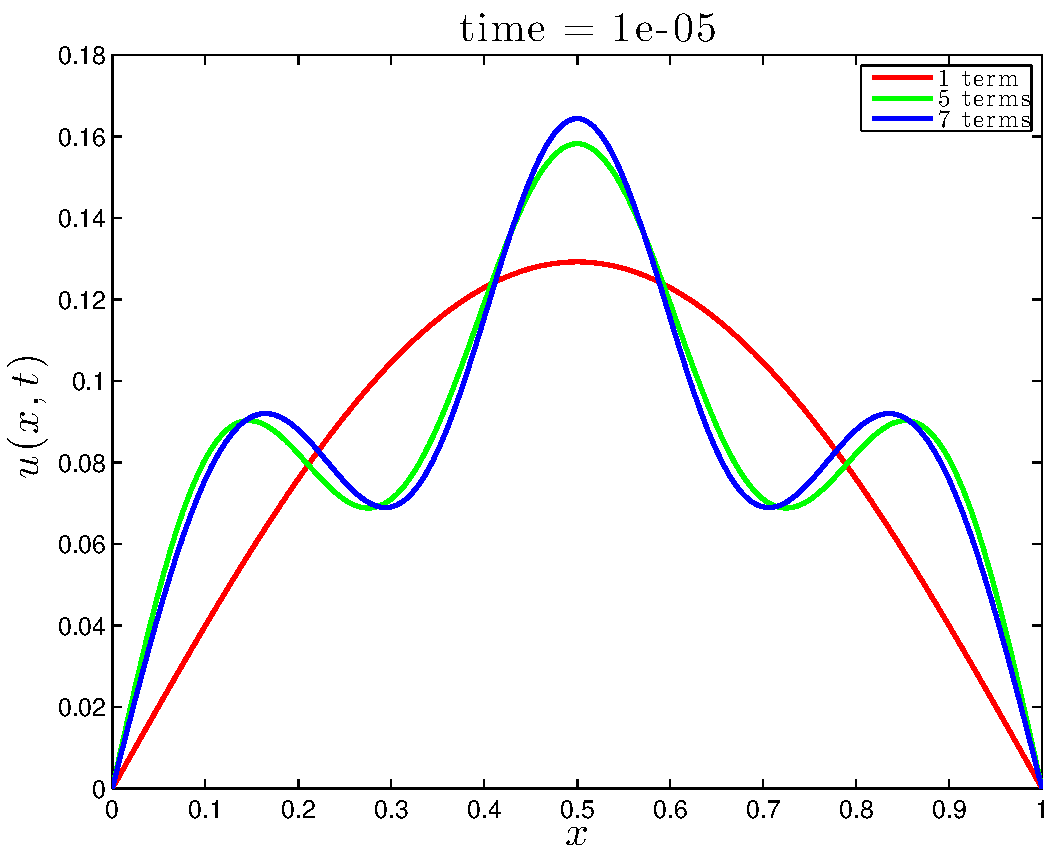
\includegraphics[scale=0.4]{fourth_b}

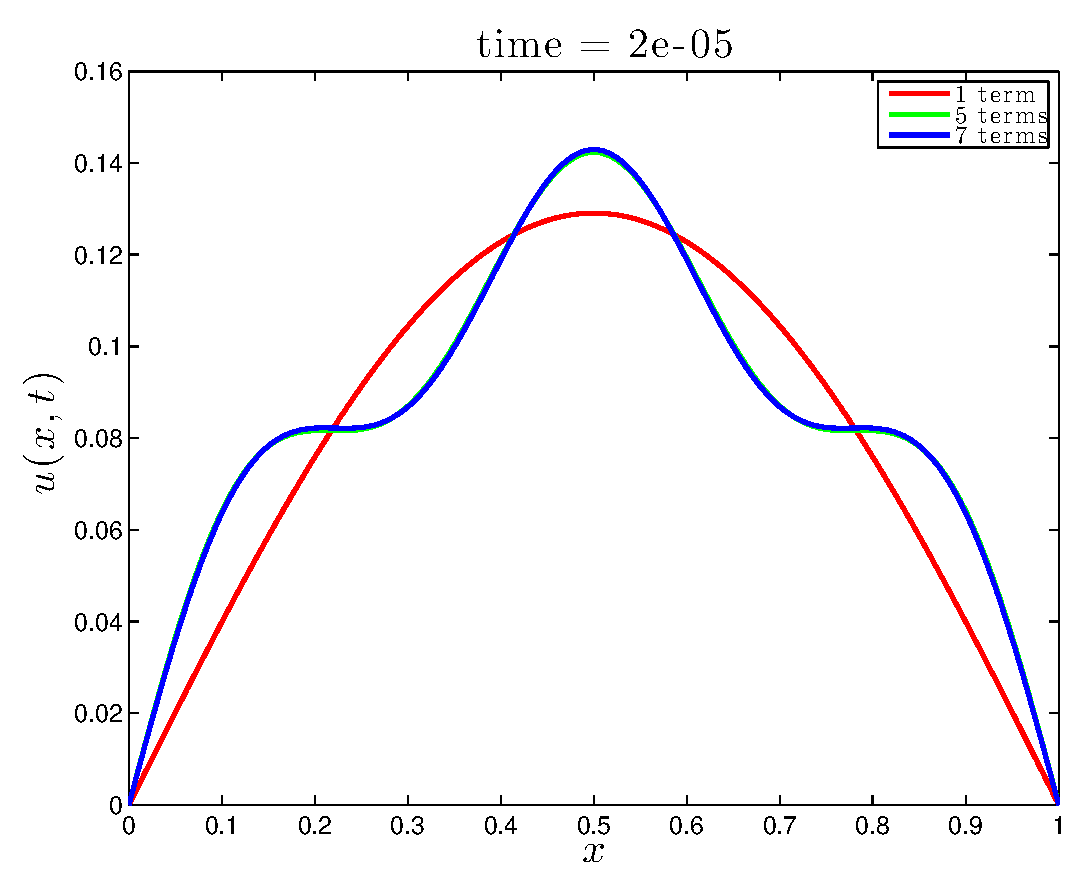
\includegraphics[scale=0.4]{fourth_c}
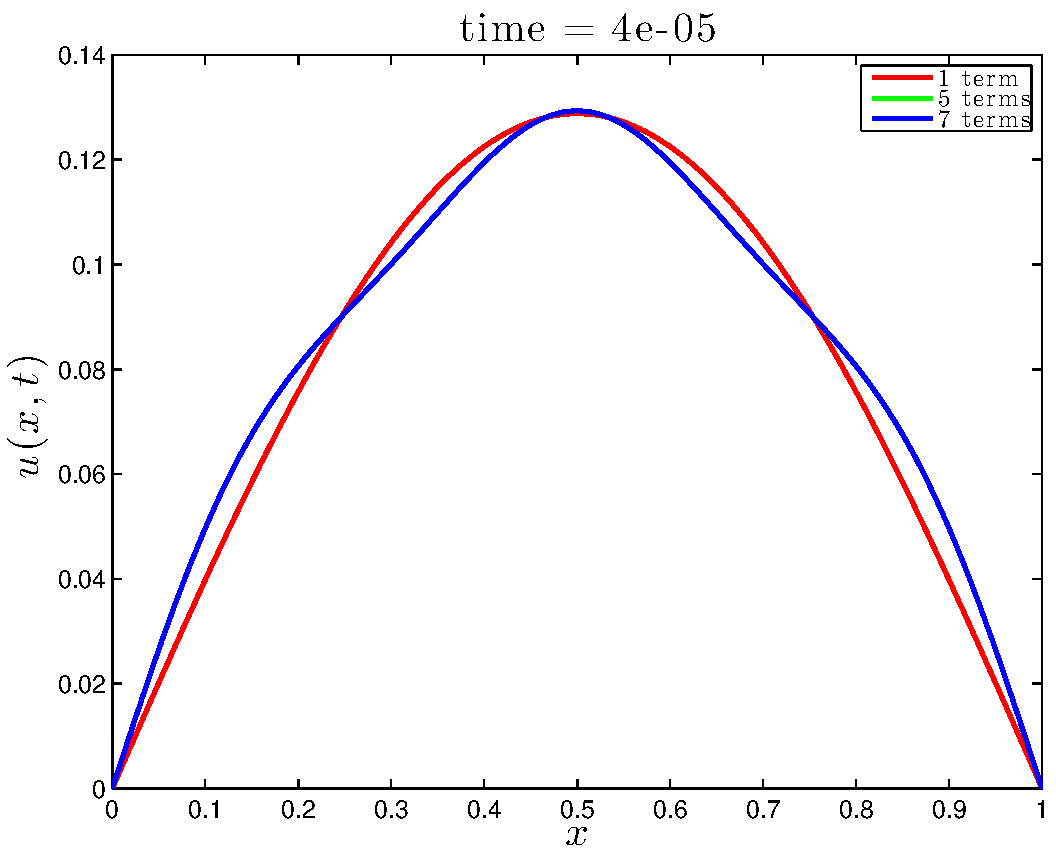
\includegraphics[scale=0.4]{fourth_d}
\end{center}
Alternatively, students may produce three-dimensional plots over the same time
span for 1, 5, and 7 terms in the Fourier series.

\hspace*{-7em}
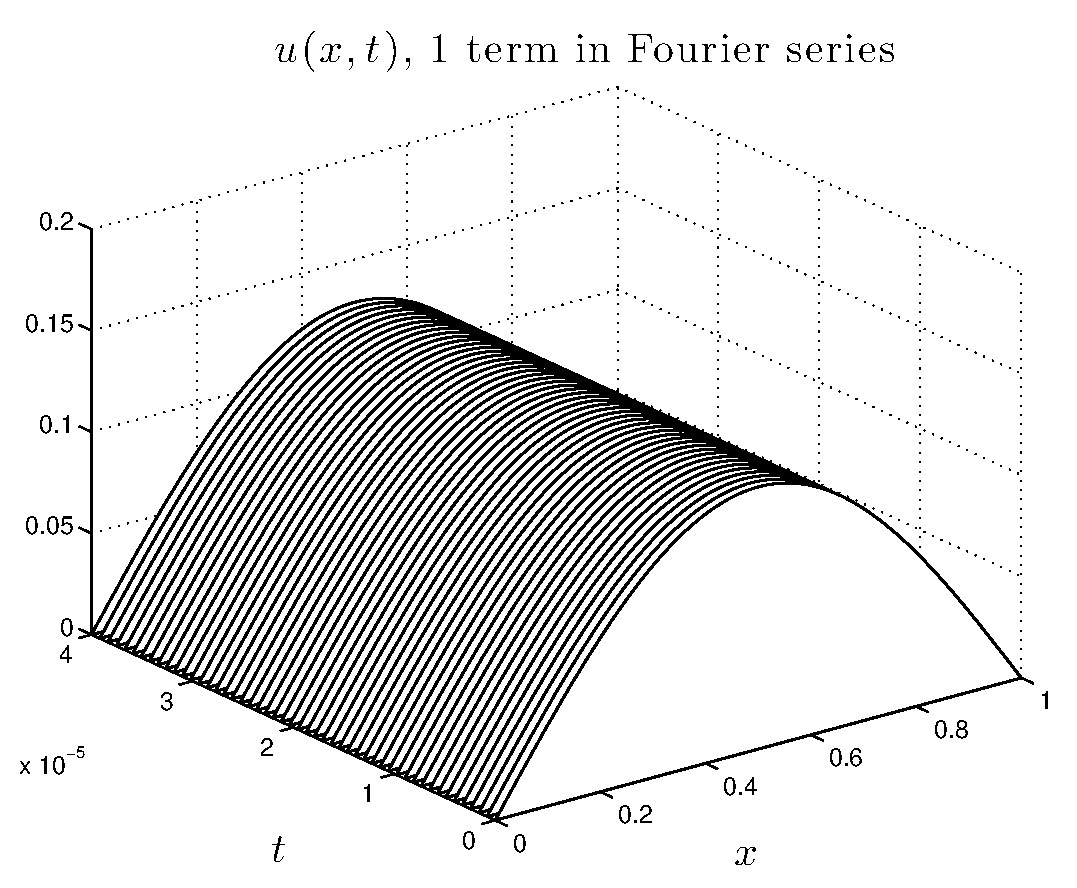
\includegraphics[scale=0.5]{fourth_wf1}
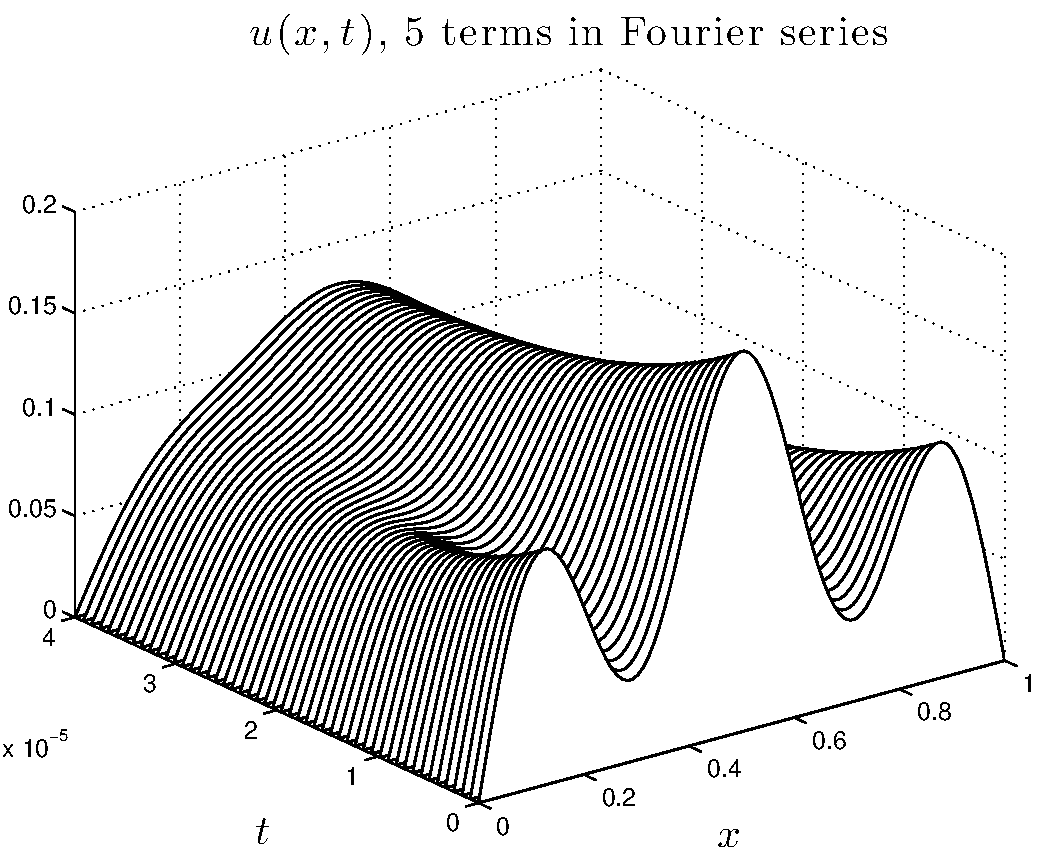
\includegraphics[scale=0.5]{fourth_wf5}

\begin{center}
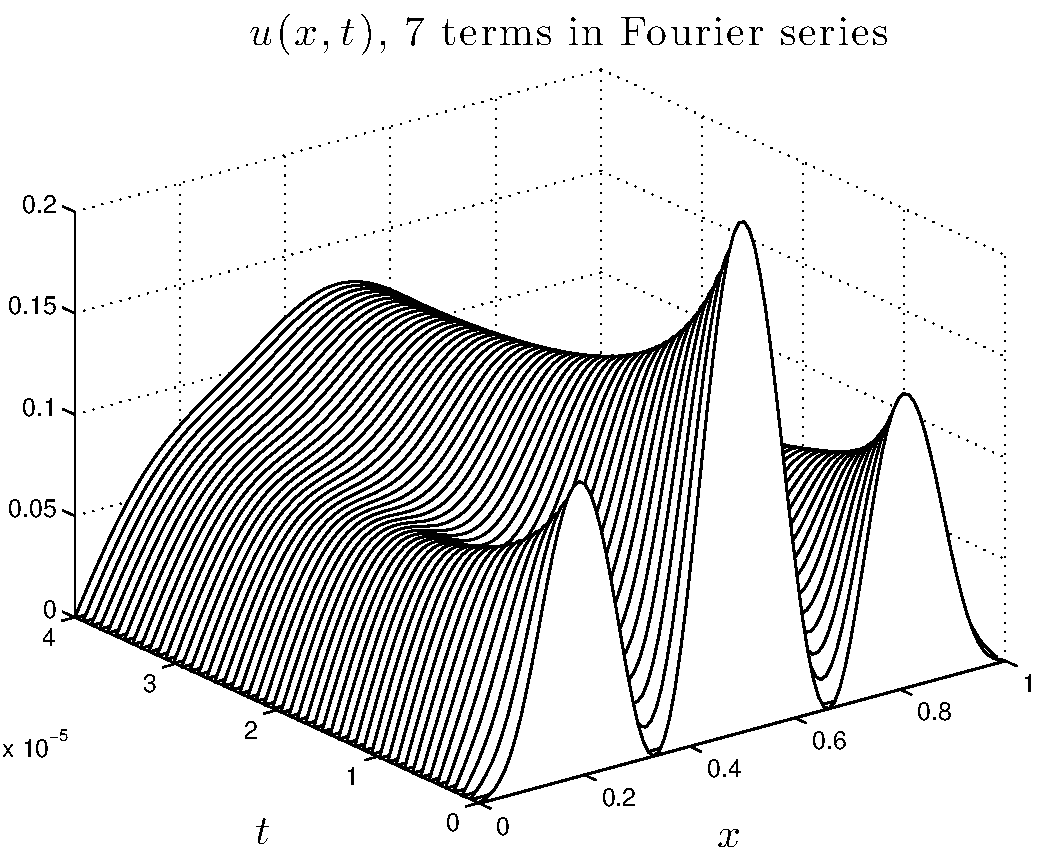
\includegraphics[scale=0.5]{fourth_wf7}
\end{center}

One can produce these plots with the following code.
\input fourth_code
\end{enumerate}
\end{solution}}{}

